% chktex-file 1
% chktex-file 29

\FILENAME

\section{Intorduction to Docker}
\label{Docker}
\index{Docker}


\subsection{Topics Covered and Learning Outcome}

\begin{itemize}

\item What is Docker?
\item What are containers?
\item Components in Docker
\item Run an example with Docker
\item Gain practical experience with Docker

  \begin{itemize}
  \item docker installation
  \item docker hello world
  \end{itemize}

\end{itemize}

\subsection{What is Docker?}

Docker is the company driving the container movement and the only
container platform provider to address every application across the
hybrid cloud. Today's businesses are under pressure to digitally
transform but are constrained by existing applications and
infrastructure while rationalizing an increasingly diverse portfolio of
clouds, datacenters and application architectures. Docker enables true
independence between applications and infrastructure and developers and
IT ops to unlock their potential and creates a model for better
collaboration and innovation.

\begin{figure}[htbp]
\centering
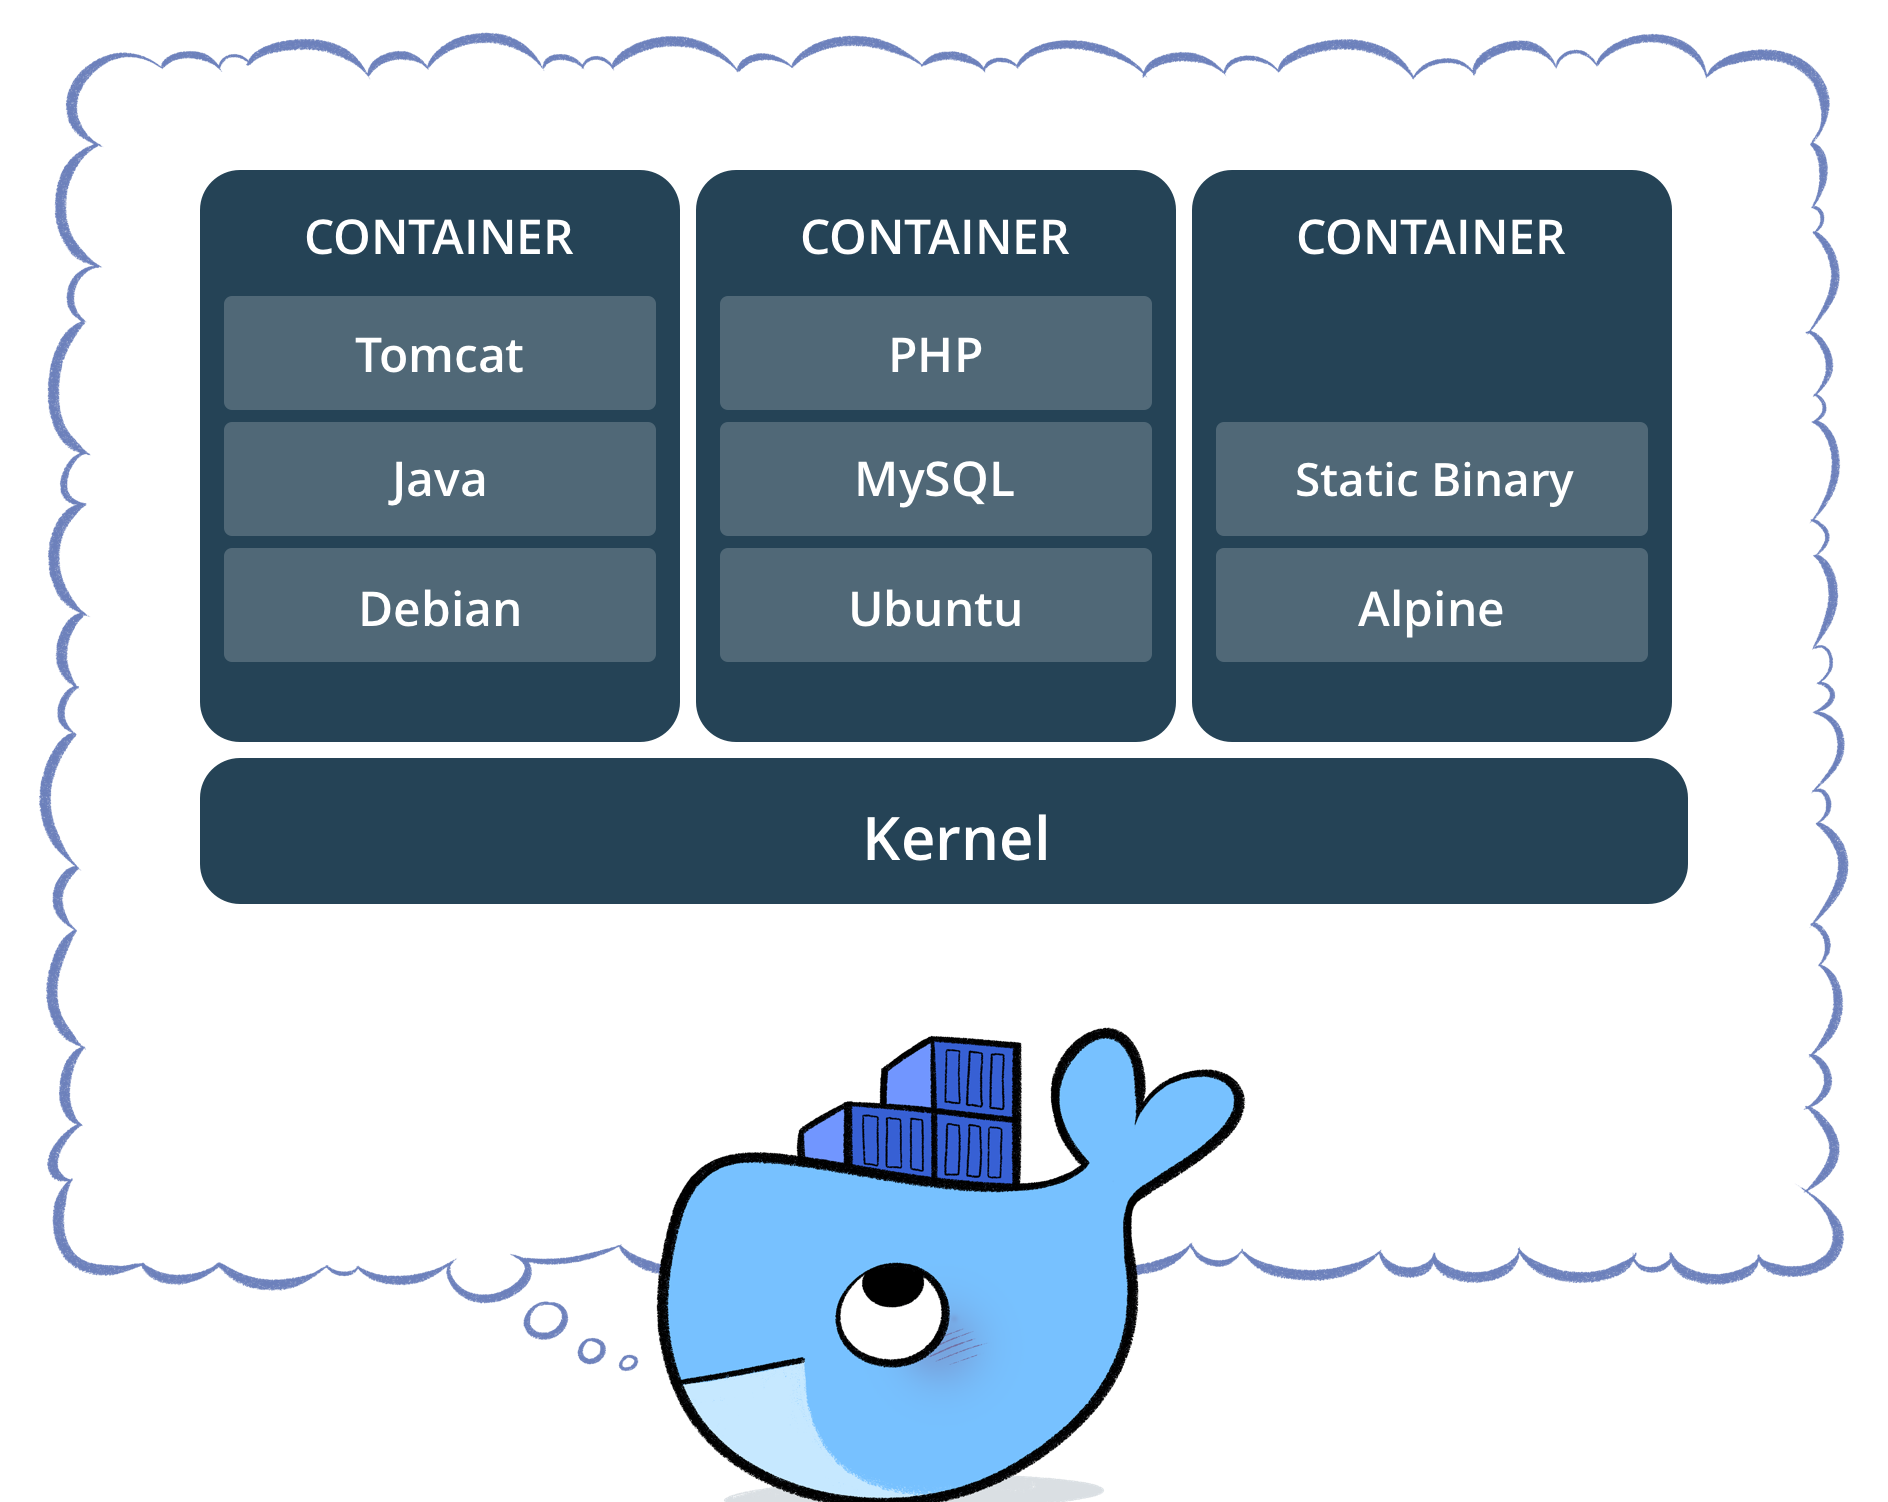
\includegraphics[width=0.7\textwidth]{docker-container.png}
\caption{Docker Containers}
\end{figure}

Image Source
\url{https://www.docker.com/sites/default/files/Package\%20software\%40x2.png}

\subsection{Install Docker}

\subsubsection{Install Docker for OSX}

In order to install on OSX, you need to do the following steps:

\begin{enumerate}
\def\labelenumi{\arabic{enumi}.}
\item
  Download \texttt{Docker.dmg} file from
  \href{}{https://docs.docker.com/docker-for-mac/install/\#download-docker-for-mac}
\item
  Start \texttt{Docker.app}
\end{enumerate}

\subsubsection{Install Docker for Windows
10}\label{install-docker-for-windows-10}

\href{https://download.docker.com/win/stable/Docker\%20for\%20Windows\%20Installer.exe}{Download
docker}

\href{https://download.docker.com/win/stable/DockerToolbox.exe}{Download
docker toolbox}

Move these downloaded files to a directory as shown below.

\begin{verbatim}
mkdir C:\Users\<username>\Documents\cloudmesh
\end{verbatim}

Replace with the username in your Windows 10 account

Example: Neo

\begin{verbatim}
mkdir C:\Users\Neo\Documents\cloudmesh
\end{verbatim}

Place all the downloaded exe files in the cloudmesh directory we created
earlier. First do the Docker installation and then do the Docker Toolbox
installation. Then you can double click the exe file and run it for
installation.

When you are doing the installation, tic mark the descriptions in the
installation saying to create shortcuts in your desktop. This way you
can load all the tools in the desktop as shortcuts.

For running you will need the \textit{Docker Quickstart Terminal} application
and it will load all the requirements and provide a terminal window in
which you can execute docker commands.

Once the terminal is loaded, it will show something like following:

\begin{verbatim}
$ <username>@<yourpc> MINGW64 ~
\end{verbatim}

For instance

\begin{verbatim}
$neo@neo MINGW64 ~
\end{verbatim}

\subsubsection{Install Docker Commuinity Edition for
Ubuntu}\label{install-docker-commuinity-edition-for-ubuntu}

In order to instal Docker community edition for Ubuntu, you first have
to setup the repository where it is located. This can be achieved as
follows:

\begin{verbatim}
$ sudo apt-get update

$ sudo apt-get install \
    apt-transport-https \
    ca-certificates \
    curl \
    software-properties-common

$ curl -fsSL https://download.docker.com/linux/ubuntu/gpg | sudo apt-key add -

$ sudo apt-key fingerprint 0EBFCD88

$ sudo add-apt-repository \
   "deb [arch=amd64] https://download.docker.com/linux/ubuntu \
   $(lsb_release -cs) \
   stable"
\end{verbatim}

Now you have configured the repository location, you can install it
after you haved updated the operating system. The update and install is
done as follows:

\begin{verbatim}
$ sudo apt-get update
$ sudo apt-get install docker-ce
$ sudo apt-get update
\end{verbatim}

To check if the Docker works, please follow the following command.

\begin{verbatim}
$ sudo docker run hello-world
\end{verbatim}

